\documentclass[conference]{IEEEtran}

\usepackage{cite}
\usepackage{amsmath}

\usepackage{framed}
\usepackage{listings}
\usepackage{algorithm}
\usepackage{algorithmic}

\usepackage{graphicx}
\usepackage{cleveref}


\begin{document}
\title{An Algebra for Robust Workflow Transformations}



\author{
\IEEEauthorblockN{Nicholas Hazekamp}
\IEEEauthorblockA{University of Notre Dame \\
Notre Dame, Indiana 46556 \\
nhazekam@nd.edu}
\and
\IEEEauthorblockN{Douglas Thain}
\IEEEauthorblockA{University of Notre Dame \\
Notre Dame, Indiana 46556 \\
dthain@nd.edu}
}

\date{18 June 2018}


\maketitle

\begin{abstract}
Scientific workflows 
are often designed with a
particular compute site in mind.
As the site changes,
the workflow needs to adjust.
These changes include 
moving from a cluster to a cloud,
updating an operating system,
or investigating failures on a new cluster.
As a workflow is moved, 
its tasks do not fundamentally change,
but the steps to configure, 
execute, and evaluate tasks differ.
When handling these changes it may be necessary
to use a script to analyze execution failure or
run a container to use the correct operating system.
To improve workflow portability and robustness,
it is necessary to have
a rigorous method that allows transformations on a workflow.
These transformations do not change the tasks, 
only the way tasks are \emph{invoked}.
%More of this
Using technologies such as containers, resource managers, and scripts 
to transform workflows allow for portability,
but combining these technologies
can lead to complications with execution and error
handling.
% still odd phrasing
We define an algebra to reason about task transformations 
at the workflow level and express it
in a declarative form using JSON.
We implemented this algebra in the
Makeflow workflow system and demonstrate
how transformations can be used for 
resource monitoring, failure analysis, and software deployment across three sites.
\end{abstract}



\section{Introduction}

% Context: Scientific workflows (give examples)
% Goal: Run on different sites, configurations. (give examples)
% Problem: Modifying workflows is hard to get right. (give examples)
% Solution: An algebra for workflow transformations.
% Implementation: How did you build it?
% Evaluation: Summarize case studies.

Scientific workflows define a set of tasks 
and their interdependencies to provide
performance, reproducibility, and portability.
Workflows are used every day in 
bioinformatics\cite{pmid20080505, pmid2231712, makeflow-examples, giardine2005galaxy, blankenberg2010galaxy, goecks2010galaxy}, 
high energy physics\cite{10.1007/978-3-540-24669-5_107, lobster-cluster-2015}, 
astronomy\cite{10.1007/978-3-540-28642-4_2}, 
and many other domains.
Workflow management systems provide support for 
expressing the required resources,
environment, and configuration for each task.
Correctly specified workflows are explicit
about required setup and environments.
Often these workflows are designed for a 
specific site, failing when
moved to different sites.


Differences between execution sites
makes porting workflows hard 
and makes debugging complex. 
It is common for workflows to
assume libraries and programs are available, 
use  applications configured for only one operating system,
or rely on unspecified configurations,
all of which fail on different sites.
Accommodating each site's configuration
requires a number of unique transformations to properly execute.
The tasks themselves do not change,
but the environment, error handling, and configuration 
may.


A typical use case is the 
need to deploy the same operating system and
software stack on several available
compute sites.
Unfortunately, each site may have a unique
operating system or lack the necessary software.
Users need a way to quickly switch between
each site, but we do not want to rewrite the 
workflow for each one.
The simple answer is to use containers,
but how do we easily apply these containers 
to tasks?
This is further complicated when each site
may use different container technologies
(i.e. Docker\cite{Merkel:2014:DLL:2600239.2600241}
and Singularity\cite{Singularity}).

The ability to combine available tools is required
to handle unique configurations and environments.
As the number and variety of tools increases, 
the complexity of combining them increases as well.
For example, if 
Singularity and a custom script
are both applied to a simple task by prepending their
commands, characteristics of execution like
exit status, provenance of files, and
the final executed command become opaque.
Properly nesting the container inside of a
script allows for differentiating failures, 
debugging, and consistent execution.
Each additional layer must become a more nuanced transformation
as nesting technologies, 
such as containers,
resource monitoring, 
and error handling,
becomes necessary.
Different combinations of tools are required
depending on the site's unique configuration.
The variable nature of required tools indicates
the importance of only applying tools to a workflow as needed, 
rather than adding them to the workflow specification at each site.

To address this problem,
we define an algebra for workflow transformations
to address the complexity of
nesting different tools and technologies.
Based on the sandbox model of execution, 
this algebra formalizes the operations
for applying transformations to tasks, 
producing new tasks.
These transformations can then be applied
in series to produce a task that incorporates
all applied transformations.
Using formalized task transformations,
we are able to precisely apply multiple transformations to a workflow 
and cleanly map to each task.

This algebra was expressed using JSON 
so that it is independent of
(and therefore portable to)
a variety of systems. 
Using this JSON expression, a driver was written
in Makeflow\cite{makeflow-sweet12} that allows us to apply transformations 
to a full workflow.
We discuss the challenges 
in applying transformations and 
how these methods can
be applied incorrectly and incompletely. 
To show the efficacy of this solution
we show several case studies. 
The first uses a Singularity container 
to provide consistent environments, 
a resource monitor to give accurate usage stats, and
a sandbox to isolate the available files and workspace.
The second shows a failure handler that captures a
core dump and converts it into a stacktrace, 
streamlining analysis and lower data transfer.
The final case study executes the same workflow on
several sites using an environment builder 
that dynamically builds required software at each task. 

\section{Background and Challenges}

% What is a workflow.
Scientific workflows are a widely used means of organizing
a large amount of computational work.  A workflow consists
of a large number of tasks, typically organized in a graph structure
such that the outputs of some tasks can be used as the inputs 
of other tasks.  Each task is a unit of work that can be dispatched
to a batch system or cloud facility and can range in scale anywhere
from a brief function call lasting a few seconds to a large parallel
application running on hundreds of nodes for several hours.
Examples of widely used workflow management systems include
Pegasus~\cite{pegasus}, 
Kepler~\cite{doi:10.1002-cpe.94}, 
Swift~\cite{swift}, 
Makeflow~\cite{makeflow-sweet12}, and many others. Figure~\ref{fig:workflow} shows an example of a typical
workflow structure.

\begin{figure}[t]
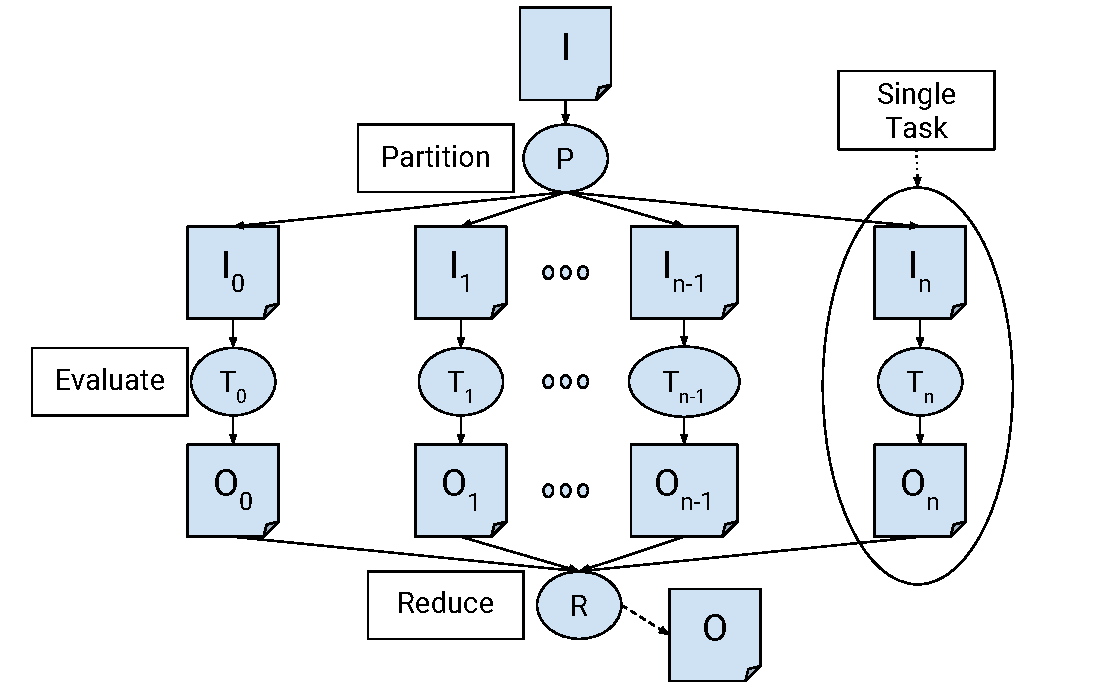
\includegraphics[width=\columnwidth]{graphics/example_workflow.pdf}
\caption{Example Workflow.}
\small
\emph{This basic workflow shows
standard split-join behavior. The first task partitions the work, the next set of tasks analyze the individual 
partitions, and the last task joins them all back 
together. Each task executes independently from each other
and are often run on batch execution systems.}
\label{fig:workflow}
\end{figure}


% Primary goal: run the app, but multiple secondary goals of tailoring, monitoring, debugging
A workflow primarily describes the researcher's work
to run a set of simulations, 
to analyze a dataset, 
to produce a visualization, etc.
However, like any kind of program, there may be a number of secondary
requirements that must be met to complete the work:
a particular software environment should to be constructed,
resource controls for the batch system will be selected,
monitoring and debugging tools should be applied to the task,
and so forth.  This might involve  
setting environment variables,
providing additional inputs, capturing additional outputs,
invoking helper processes, and more.

% These actions require modifying the workflow, but can get confused with the primary task and make it difficult to port.
The first version of a workflow, constructed at a particular computing site,
may have all of these aspects intertwined with the definition of the
tasks to be done.  
The application may depend upon
software environments installed in fixed paths in a shared filesystem.
Environment controls may be set within individual tasks.
Resources may be
hard coded for a particular batch system
The graph structure may reflect
the current set of debugging tools enabled.  
While this may work well at the
first site, it may become necessary to move the workflow to another
site in order to improve performance, increase scale, or to apply the workflow in a new context.
All these site-specific controls are unlikely to work in the new context,
and the receiving user is then stuck with the problem of disentangling the
core code from the local peculiarities.

% Idea: wrappers
An appealing approach to this problem is to define 
simple modifications that can be individually applied to tasks
(transformations) in order
to achieve specific local effects.  For example, one might have a transformation
to run a task in a container environment, another transformation to perform monitoring
and troubleshooting, and a final transformation to configure a software environment
for the local site.  With this approach, the scientific objective of the workflow
can be expressed in a portable way. 
A set of external transformations are used to
modify the tasks as needed for the local site.  Porting a workflow from one site
to another becomes the simple job of adjusting a few transformations rather than
rewriting the workflow from scratch.  If it is necessary to transform
the workflow in a new way, a new transformation can be written and shared
with others so that it can be applied to many workflows.

% Challenges of wrappers
However, our experience is that designing and using transformations
is not so easily done. What may seem like a simple and obvious
transformation can end up creating complex interactions and
incorrect results.  As a simple example, suppose that
we want to run each task inside a Singularity
container named {\tt centos.img}.
At first, this sounds
as simple as prepending {\tt singularity run centos.img} to each
command string then running the task.  While this 
works in limited cases, the general case for workflows
with complex task definitions fails.  There are several reasons for this:

%\begin{itemize}
    %\item 
    {\bf Substitution semantics.} 
    Using basic string substitution to embed one command 
    inside another often complicates execution.  
    Commands that use 
    input/output redirection,
    consume files,
    or change the environment 
    collide using basic substitution.
    Addressing this uncertainty with shell quoting only 
    further complicates the matter, and may
    change the execution.

        
    %\item 
    {\bf Workflow modifications.}
    Applying a transformation to a task not 
    only changes the individual task, 
    but may also have an effect on the 
    global structure of the workflow.  
    A command transformed by a container 
    now has an additional input ({\tt i.e. centos.img})
    which must be accounted for as a 
    dependency in the workflow.
    Container images are large and affect the 
    scheduling and resource management of the workflow.  
    In a similar way, the container produces additional 
    outputs which must be collected and managed by the
    workflow.
    
    %\item 
    {\bf Namespace conflicts.}
    Transformations can modify 
    the local filesystem namespace.
    Log files with fixed names, 
    temporary generated files, 
    files based on task input files, 
    or modifications to the working directory 
    all alter the task and the workflow.
    These actions blindly modify files 
    outside the workflow or cause 
    race conditions with other concurrent transformations.
    Since it is not always possible to alter these
    hard-coded paths into unique filenames,
    collisions are inevitable.
    
    %\item 
    {\bf Troubleshooting complications.}
    The exit semantics of a transformed task are complex 
    as it is not sufficient for a transformation to simply
    return the task's integer exit status.
    Each exit status should be differentiated,
    as transformations may fail separately.
    For example, preparing the environment may fail because a
    necessary software dependency is not present,
    a container may fail when pulling the container image over the network, or 
    a resource monitor may exit when resources are exhausted.
    In each of these cases, we must have a means of distinguishing
    between \emph{transformation failure} and \emph{task failure}.
    When multiple transformations are applied, the result of the
    task looks more like a stack trace than a single integer.
%\end{itemize}


% Concl: We need an algebra
To address these challenges, we need a more
rigorous way of defining tasks and the transformations
on those tasks such that any valid transformation applied
to any valid task gives the expected result in a
way that can be nested.  In short, we need an algebra
of workflow transformations in order to make scientific
workflows more robust, portable, and usable.

%\input{outtake_background.tex}

\section{An Algebra of Workflow Transformations}

We designed a formal abstraction
to accommodate the execution behavior
of various tools. 
This formalism isolates each transformation 
for consistent execution,
allowing for organized nesting. 
In particular, our abstraction describes how to define 
a transformation for a given tool, 
as well as aspects of execution to consider. 
Transformations are based on the 
sandbox model of execution, 
which describes all aspects of execution 
for which a transformation is responsible.

\subsection{Notation}

For the purpose of expressing tasks and transformations in a
precise way, we use a notation that is based on
JavaScript Object Notation (JSON).
In addition to the standard JSON elements of 
atomic values (\verb$true$, \verb$123$, \verb$"hello"$), \emph{dictionaries} \verb${ name: value }$, and \emph{lists} \verb$[ 10, 20, ... ]$,
we add:

\begin{itemize}
    \item {\tt let X = Y} is used to bind the name {\tt X} to the value {\tt Y}.
    \item {\tt define F(X) = Y} defines a function {\tt F} that will evaluate to the value {\tt Y} using the bound variable {\tt X}.
    \item Simple expressions can be built up using standard arithmetic operators and function calls on values and bound variables.
    \item {\tt eval X} evaluates the expression X and returns its value.
\end{itemize}

Using this notation, a single task ($T1$) in a workflow
is expressed in JSON like this:

\begin{figure}[H]
\begin{framed}
%\small
\begin{verbatim}
let T1 = {
 "command": {
   "pre":[ ],
   "cmd": "sim.exe < in.txt > out.txt",
   "post":[ ], 
   },
 "inputs"     : [ "sim.exe", "in.txt" ],
 "outputs"    : [ "out.txt" ],
 "environment": {},
 "resources"  :
   {"cores":1, "memory":1G, "disk":10G }
}
\end{verbatim}
\end{framed}
\label{basic-task}
\end{figure}

Note that the schema is fixed.
Every task consists of a command with a \verb$pre$, \verb$cmd$, and \verb$post$ component, a list of input files, a list of output files,
a dictionary of environment variables, 
and a dictionary of necessary resources.  
Also note that the formal list of
inputs and outputs is distinct from the command-line to be executed,
as guessing the precise set of files needed from 
an arbitrary command-line is difficult.  For example,
a program might implicitly require a calibration file {\tt calib.dat}
and yet not mention that on the command line.  
The base task's list of inputs
and outputs is drawn from the structure of the DAG by the workflow
manager.



\subsection{Semantics}
\label{sec:sandboxing}

Makeflow allows for tasks in this form to be executed on a wide
variety of execution platforms, including traditional batch
systems (such as 
SLURM\cite{Jette02slurm:simple}, 
HTCondor\cite{condor-hunter}, 
and SGE\cite{Microsystems:2001:SGE:560889.792378}), 
cluster container managers, and cloud services.
Because each of these systems differ in considerable ways,
it is necessary to define precise semantics about the
execution of the task and the namespace in which it lives.
Once these semantics are established, it becomes possible
to write transformations that work correctly regardless of the underlying system.
To accommodate these varied systems, we introduce the
sandbox model of execution.

The {\bf sandbox model} of execution isolates the environment 
and limits interactions to only specified files.
Isolating the task to run only the specified environment allows for higher
flexibility about where the task can run as well as increasing the reproducibility
of execution. Limiting the locally available files helps
prevent undocumented file usage, enforcing accuracy of the
file lists.


Applying a sandbox to a task is 
a multi-step process for ensuring consistent environment creation:
\begin{enumerate}
    \item Allocate/ensure appropriate space for execution, based on resources.
    \item Create sandbox directory.
    \item Link/copy inputs to ensure correct in-sandbox name, based on inputs.
    \item Enumerate environment variables based on the specified environment.
    \item Run task defined command, 
    using \emph{pre}, \emph{cmd}, and \emph{post}.
    \item Move/copy outputs outside of sandbox with appropriate out-sandbox name, based on outputs.
    \item Exit and destroy sandbox.
\end{enumerate}


\begin{figure}[H]
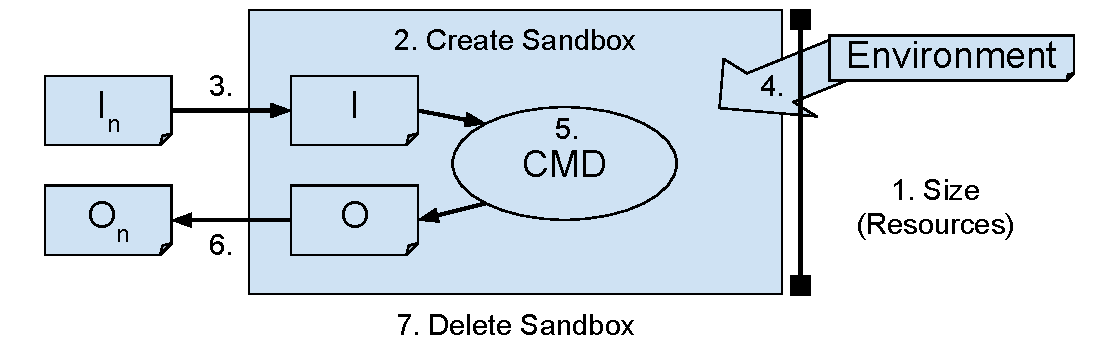
\includegraphics[width=\columnwidth]{graphics/sandboxing_short.pdf}
\caption{The Sandbox Model of Task Execution.
This shows the different steps needed to isolate
the task from the underlying workflow environment
to prevent side-effect on the environment and 
filesystem.}
\label{fig:sandbox}
\end{figure}


\begin{figure}[t]
\begin{framed}
%\small
\begin{verbatim}
define Singularity(T) 
{
 "command" : {
 
   "cmd": "singularity run image " +
           T.script + " > log." + T.ID
         
 }
 "inputs"   : T.inputs + 
              ["image", T.script],
 "outputs"  : T.outputs +
              ["log."+T.ID],
              
 "resources" : {
 
 
   "disk"   : T.resources{disk} + 3G
 }
}
\end{verbatim}
\end{framed}
\caption{Abstract {\tt Singularity} Transformation}
\small
\emph{Describes the Singularity command, added files
(such as image and output log), and increases
the required disk space. Note, several of the
variable are unbound, and will be resolved when
applied to a task. Unaltered fields are left
undefined.}
\label{sing-wrap}
\end{figure}



\subsection{Transformations as Functions}

A transformation is an abstraction of a task,
and provides the information needed
to translate a raw program invocation into 
a properly defined task. 
A transformation contains the same fields defined in a task: 
a command, inputs, outputs, 
resources, and environment.
However, it is an incomplete task with 
unbound variables that are resolved 
when applied to a task as a function.

\Cref{sing-wrap} illustrates  
Singularity written as a transformation.
As mentioned above, the generic definition of
the transformation contains unbound variables
such as {\tt T.cmd}, {\tt T.inputs}, and
{\tt T.outputs}. 
When the transformation is 
applied to a task, those variables
are bound from the task's structure.
Singularity requires
additional space (3G) to account 
for the Singularity image. 
Here, resources are not defined as
a static value, but in addition the to 
underlying resource. 
Additionally, the Singularity transformation 
does not
define an environment, so it is left out. 


\begin{figure}[t]
\begin{framed}
%\small
\begin{verbatim}
eval Singularity(T1) yields
{
 "command": {
   "pre":[ ],
   "cmd": "singularity run image " +
          "t_ID.sh > log.ID"
   "post":[ ],
 },
 "inputs"   : ["sim.exe", "in.txt", 
               "image", "t_ID.sh" ],
 "outputs"  : ["out.txt", 
               "log.ID"],
 "environment" : {}
 "resources" : {
   "cores"  : 1, 
   "memory" : 1G, 
   "disk"   : 13G,
  }
}
\end{verbatim}
\end{framed}
\caption{Resulting task of applying {\tt Singularity} to {\tt T1}.}
\small
\emph{The transformed task has all of the variables bound.
The file lists have combined the previously defined files
with the files added by {\tt Singularity}.
The resources are resolved and the required values account
for the original task and the transformation.}
\label{sing-task}
\end{figure}


The resulting task of evaluating 
\verb$Singularity(T1)$
can be seen in \Cref{sing-task}.
The previously unbound variables have
been resolved, such as {\tt T.inputs}
becoming {\tt ["sim.exe, "in.txt"]}.
The values that were not defined or
extended by \verb$Singularity$ were
resolved from the underlying task,
such as {\tt cores} and {\tt memory}.
Importantly, to create a valid task
even empty fields like $pre$, $post$,
and $environment$ are still specified, 
allowing for evaluation and additional
transformations to be applied.

If you look carefully at \Cref{sing-wrap}
you will notice two variables not
bound by the underlying task
directly, {\tt T.script} and {\tt T.ID}.
As part of the abstraction, the 
underlying task is emitted as a script
that is called in place of the command,
creating {\tt T.script}.
The ability to treat transformations as functions 
is achieved by isolating 
each transformation as a separate process.
Isolating a transformation provides 
several key benefits:
clearly defined ordering of transformations,
instantiated environments persist only 
in that process and its children,
and exit status can be attributed 
at each level to track failures.
In practice this is achieved by 
producing a script that
defines the task, as seen in \Cref{task-script}.

The second variable, {\tt T.ID},
is key to this method's success, as 
the ability to uniquely identify
each task provides a clear
mapping to the workflow.
A unique identifier is created
using the checksum of the
current task, which incorporates the
command, input files' names and contents,
output files' names, environment, and
resources. 
This identifier is used to identify the output
script and can be used by the
transformation to uniquely identify 
files in the workflow.
Additionally, as applying a transformation
produces a new task, the identifier 
is updated after each transformation.

\begin{figure}[h]
\begin{framed}
\small
\begin{verbatim}
#!\bin\sh
#ID TASK_CHECKSUM

# POST function
POST(){
  # Store exit code for use in analysis.
  EXIT=$?
  
  # Run post commands.
  
  # Exit with stored EXIT which may
  # have been updated by post.
  exit $EXIT
}
# Trap on exit and call POST.
trap POST EXIT INT TERM

# Export specified environment.

# Run pre commands.

# Run core command.
sim.exe < in.txt > out.txt
\end{verbatim}
\end{framed}
\caption{Script created when evaluating {\tt Singularity(T1)}.}
\label{task-script}
\end{figure}


\subsection{Applying the Sandbox Model}

This creation of a script from a task
focuses on isolating just the transformation,
but relies on finalization of the task sandbox
laid out in \Cref{sec:sandboxing}.
To consistently apply the sandbox model to a task
we define a sandbox procedure to produce a script
that creates a sandbox, handles files, and runs
the command. This procedure is applied to a 
task prior to execution to isolate the task to 
a single sandbox directory.

This begins with 
creating a unique identifier, based on the task checksum.
The identifier is used to create the 
sandbox and script names used in execution. In the 
script a {\tt POST} function captures
the exit status, executes {\tt post} commands, and
returns the outputs. 
This function is set as a trap to
also analyze failures.
Next, the sandbox is created and 
inputs are linked into it. 
The process changes directories,
exports the environment, and
runs the {\tt pre} commands.
After this the environment is setup,
the task {\tt cmd} can run.


\section{Transformations in Practice}

In applying the above algebra, there are
design considerations to be made.
To maintain the ability to nest several
transformations together, it is important
to consider the naming conflicts, the
importance of differentiating {\tt pre},
{\tt cmd}, and {\tt post}, file management,
resource specification, and how the 
environment of a task is extrapolated.

\subsection{ Composability versus Commutability }
An important aspect of this algebra is the ability
to reason about how the combinations of
different transformations interact and if they 
can be applied to created a valid task.
Using the previously defined application of
transformations we find that the set of transformations
are composable, but not commutable.
These transformation are not commutable because
the ordering in which they are applied changes the core 
evaluation of the task.
This is by design, to allow for the differentiation
of transformation ordering.

Transformations, in general, are composable.
Any transformation can be
applied to any task and produce a valid task,
with the exception of static name collisions.
A static name collision can result when
an application uses hard-coded or 
default names for files, 
careless naming, or even randomly
generated names.
Running a single transformation at a time 
may not cause a collision,
but nested transformations and concurrent tasks 
make collisions inevitable, 
as is often seen with output logs
and files sharing names between tasks.

Naming is resolved at the local level by detecting
when applying a transformation 
creates overlapping names.
If collisions are detected, the 
transformation is not applied and
a failure is returned.
Though this restricts some combinations, 
this can be overcome by 
better understanding the application
and using options to 
produce unique files.


However, if the same restrictions were
applied to tasks across the workflow,
transformations with static names would
be prohibited entirely.
As this may be inevitable,
static files may be remapped
to a unique name in the workflow.
As each task is isolated in a sandbox, 
static files can be renamed when moving to the 
global namespace using the task identifiers. 
Remapping of the file relies on
a more verbose file specification as
a JSON object instead of a string filename.
JSON object specification enables the wrapper
to specify an \emph{inner\_name}, 
specifying the name inside the sandbox,
and the \emph{outer\_name},
specifying the name in the workflow context. 
An example of how this would look with
a statically named file can be seen in 
\Cref{json-file} which defines a resource
monitor transformation.

\begin{figure}[h]
\begin{framed}
\small
\begin{verbatim}
define RMonitor(T) {
 "command" : [
  "cmd": "rmonitor -- " + T.script
 ]
 "inputs"  : T.inputs + ["rmonitor",
               T.script]
 "outputs" : T.outputs +
              [{"outer_name="summary."+ID, 
               "inner_name"="summary"}]
}
\end{verbatim}
\end{framed}
\caption{Verbose JSON object file specification.} 
\small
\emph{In this example the resource monitor uses
a statically name default summary, "summary".
In this case, the the summary 
file is statically named, but will collide in
the global workflow context. To avert this
collision the file is specified with its 
static inner\_name, and a unique outer\_name
using the task's ID.}
\label{json-file}
\end{figure}


\begin{figure*}[t]
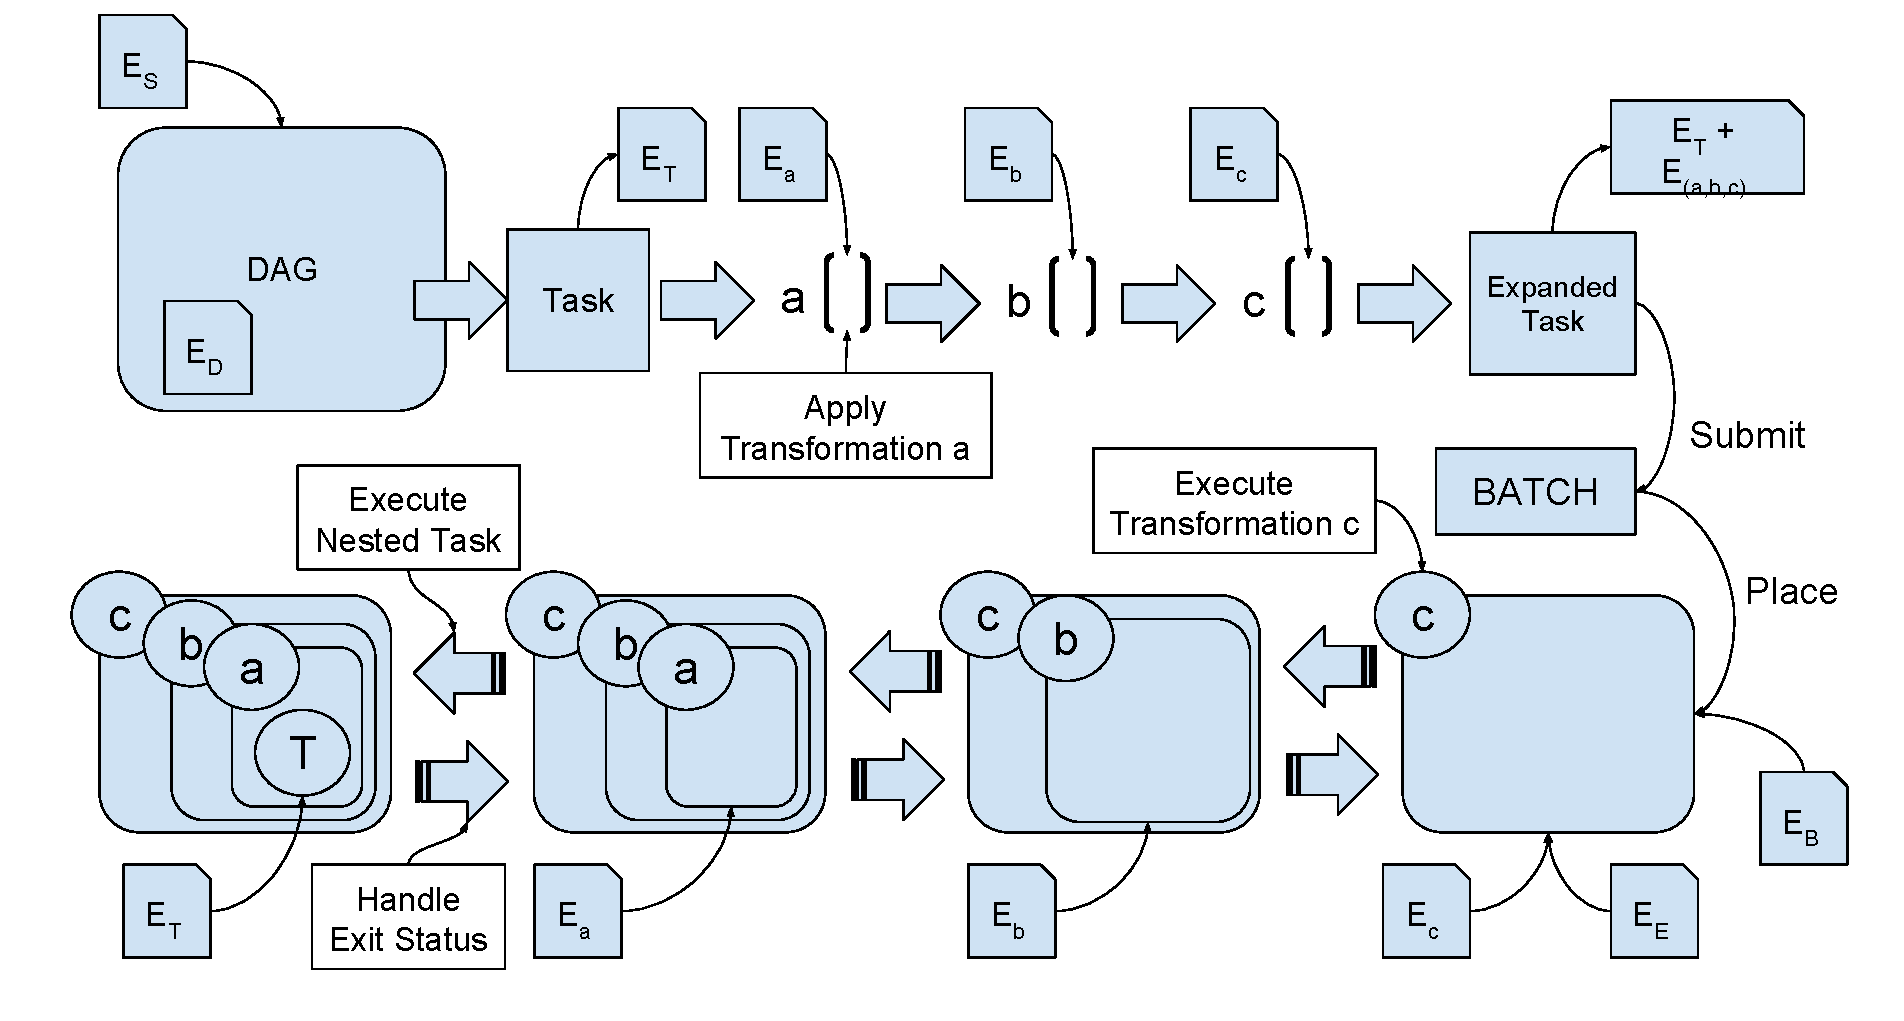
\includegraphics[width=\textwidth]{graphics/environment_extrapolation_pwrap.pdf}
\caption{General approach to Sandbox model of execution}
\small
\emph{The environment that exists at task execution is
the result of several sources. 
The environment starts at the DAG where 
variable are resolved internally and from the host machine.
These values define the task's initial environment.
Transformations are applied to this task which extend the
environment, but are only applied at execution. 
At the execution site, the environment is
defined by the execution node and batch system.
As execution starts, each transformation is
applied and invokes its environment, limiting 
their affect to that transformations execution.}
\label{figure:env-extrap}
\end{figure*}



\subsection{Command Description}

Commands express the setup, execution, and post processing
of a task. 
Commands are broken up into three parts, 
${pre}$, ${cmd}$, and ${post}$
based on the command structure outlined.

${Pre}$ is a set of commands that run prior task invocation
and setup the task sandbox. 
This includes setting environment variables, 
configuring dependencies, and loading modules or software.
For example, a Docker transformation would use ${pre}$ to load or pull images. 

${Post}$ is a set of command that run after task invocation
and is used to 
handle failure by interpreting or masking them,
create outputs to prevent batch system failures from missing files,
or validate correctness of outputs. 
${Post}$ can differentiate 
docker failing to load an image from
task execution failure, 
allowing more nuanced debugging. 

The ${cmd}$ string outlines the context in which
the underlying command is invoked.
${Cmd}$ outlines how the underlying task is called
and isolates the effects of the calling transformation.

A benefit of separating the command into these parts
is that it allows us to differentiate the failures or 
problems that result from each part.
This is useful when determining that the setup of 
your container failed so the task should not run 
or to prevent the failure of $post$ analysis from 
indicating a task failure falsely.
This separation also allows for each transformation
to be clearly expressed in a script, 
enabling simplified debugging.



\subsection{File List Management}

As transformations are applied, the list of inputs and outputs grows. 
It is key for the correct organization of transformations that the 
set of required files is outlined by the task structure
allowing the submitting system to confirm required inputs
and verify expected outputs.
It is possible for a transformation to rename or mask an existing 
file in the list.
By doing so, the transformation changes the 
context of the task when evaluated.
This can be done to allow for redirecting shared files or when using
installed reference material.
Maintaining a correct set of files helps
prevent task collision.
This information can also map a
$pre$ or $post$ application onto the files, 
estimate the space needed for execution,
or log these files for later analysis.


\subsection{Resource Provisioning}

The resources define the necessary allocation for proper task execution. 
This value is extended and augmented by transformations 
as the context and required resources change.
Commonly, as transformations are applied, 
additional disk space is needed to store new files
(like container images). 

Resource provisioning may not only be additive 
as the transformations are applied,
but also maximal.
This is typically the case used for cores.
The number of cores does not expand as
transformations are added, but reflects
the largest number of cores needed by any
transformation.
For example MPI utilizes a static number of cores, 
and to reflect that the resources specification
uses the maximum of the provided value and the previous
resource specification. 
The value of the resources required for a task 
tracks the largest set of each resource.
After the transformations have been applied, 
the final task contains a single specification 
reflecting the total expected usage.



\subsection{Environment Elaboration}

%GIVE INTRO TO ENVIRONMENT HANDLING

An important aspect of a task is the environment
where the task is executed.
The environment defines a variety of values
that control things such as available executables,
required libraries and values,
or even available machines on a cluster execution node.
However, the environment is often overlooked
or ignored by the researcher,
which can cause corruption, errors, and failures.
This can be addressed directly on a single site,
but as more sites are utilized managing these environments
becomes unrealistic.
Here we will discuss how the task environment is defined, 
when transformations are applied, and how the
final environment is resolved at execution.

The environment provided to a task varies between sites
and evolves as a task is transformed and evaluated.
The workflow is executed in the context 
of the submitting machine's environment (${E_S}$). 
As the workflow is evaluated,
the environment is defined internally and from ${E_S}$,
resulting in ${E_D}$.
Tasks are created and 
the environment that is specified by the task 
is derived from ${E_D}$, resulting in ${E_T}$. 
${E_S}$ is not included as variables would be
incorrect or reference non-existent programs, libraries, and values
at execution.

After the task is produced, 
transformations are applied that may 
append, update, or mask the provided variables.
As a transformation is applied, ${E_T}$ is 
written out to a script.
The transformation can also use the values set
in ${E_T}$ to evaluate its environment.
Applying these transformations produces
a chain of environments ${E_{Tr}}$ 
(${E_a}$, ${E_b}$, ${E_c}$ in \Cref{figure:env-extrap}) 
as a result. 

Tasks are placed on an execution node. 
The environment on the execution site
varies from that of the submission site 
and is influenced by the batch system and execution node. 
The batch system environment(${E_B}$) provides
information about the assigned machines, available cores, and location of
software modules and may be crucial 
for applications that use MPI or modules. 
The execution node environment (${E_E}$) 
defines information such as 
local disks and available hardware.

The simple method of applying the environment is to 
apply all variables either 
at the beginning of execution or 
just prior to the task invocation. 
If applied initially, there are likely uninstantiated
or unbound dependencies. 
If just prior to task execution, the context 
of each layer is evaluated using incorrect values or software.
Both ultimately lead to a disconnect 
between the intended and the actual environment.
To prevent this, as tasks are invoked 
each transformation creates a process
that only applies the specified environment,
limiting the environment's scope.
Some transformations, such as containers, 
wipe or mask the provided environment.
As transformation environments are applied, 
this should be taken into account, 
as the order and manner environments are instantiated 
may not carry through each transformation.


\section{Applications of Transformations}

We will now look at several example applications of
transformations and how they can be used to improve the portability and robustness of workflows.

\subsection{Sandbox Transform}

A sandbox transform creates a directory,
transfers files, and runs the command 
of the task.
This simple lightweight transformation isolates
the execution namespace from the workflow namespace,
which allows for file renaming.
The sandbox is removed after successful execution,
which eliminates local unspecified files from
polluting the workflow namespace and disk quota.
If a task does fail, the sandbox can be captured
and analyzed.

\subsection{Container Transform}

A container transform utilizes the whole
command structure.
A container $pre$ command is used to pull down
or unpack containers.
This is done separately to 
differentiate failure of initialization
from the invocation.
A container $cmd$ invokes the container with the 
nested command, which creates it own isolated process.
Finally, a container $post$ command cleans
up container images, reporting exit status.

Calling the nested command from the container
isolates the container arguments from the shell
script invoked. This prevents issues with 
differentiating arguments, isolating file
redirects, and instantiating an environment
inside the container.
Containers can also mask the execution environment,
which can prevent an environment specified earlier from
existing inside the container. 
Containers often increases the required resources
to account for additional files,
like container images.

\subsection{Resource Monitoring Transform}

A resource monitor transform measures the utilized resources 
during task execution. 
If limits are specified, 
the monitor will stop the task and 
report if the resources are exceeded. 
As the resource monitor relies on the 
expected resources, it can utilize the 
adjusted specification to adapt
as transformations add required resources.
Other functionality includes 
monitoring the files that are accessed and 
creating a time series of the
utilized resources.
The resource monitor uses the $cmd$ 
to track the process. 
The resource monitor benefits from the 
sandbox directory as the isolation allows 
the sandbox to be monitored for disk usage.
This does not increase the resources
but is used to enforce them.
In addition to the executable and usage summary, 
the resource monitor creates additional outputs
such as the list of accessed files and 
resource usage time series, all of which
are added as outputs.


\begin{figure*}[t]
\begin{minipage}[t]{0.17\textwidth}
  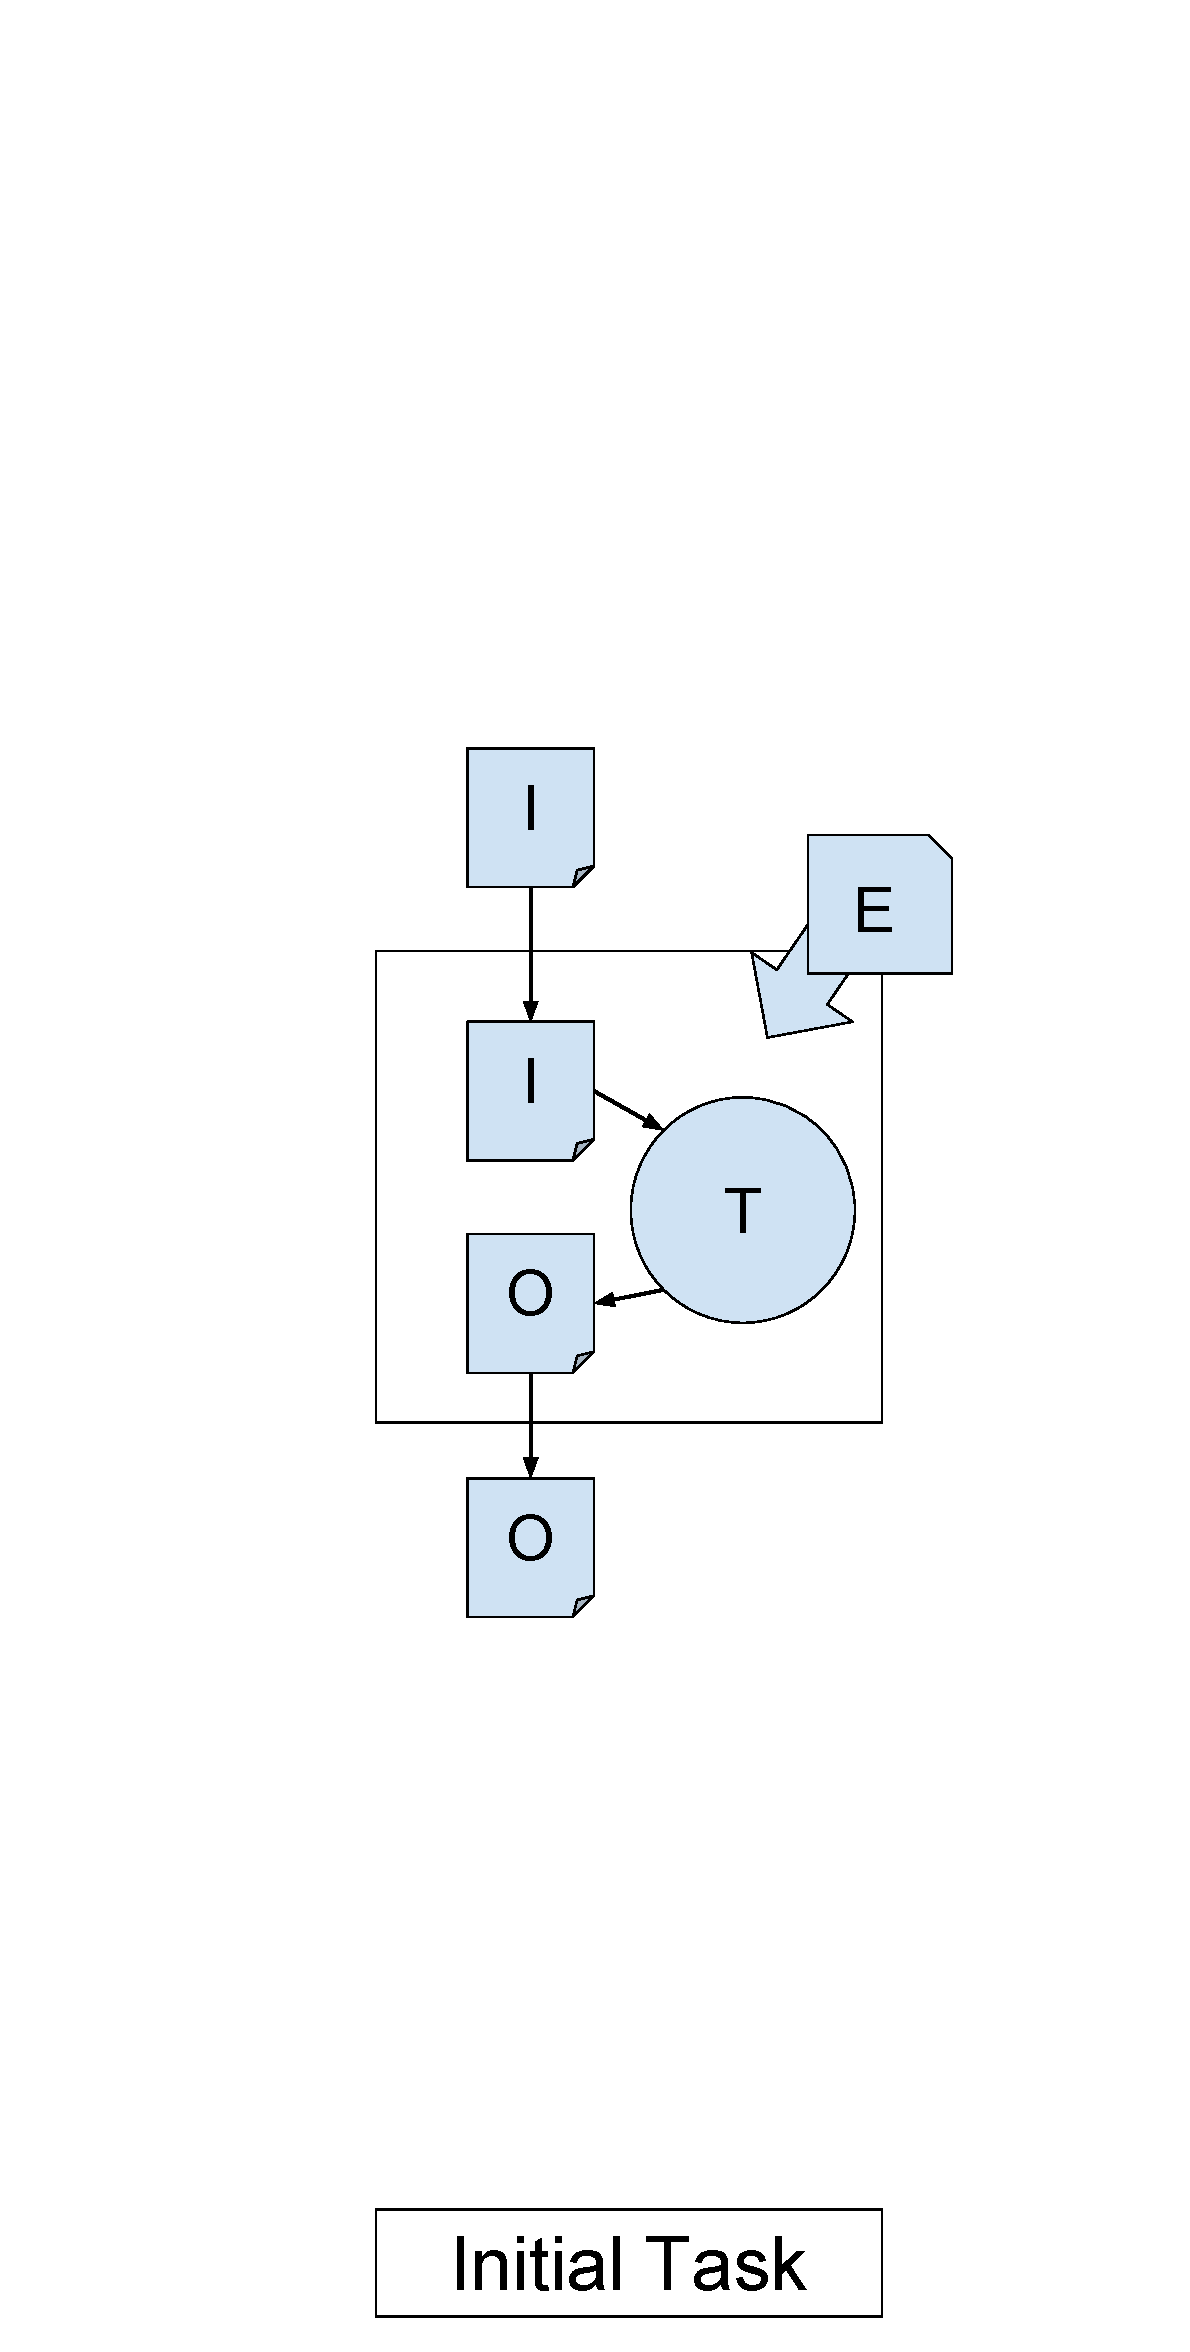
\includegraphics[width=\textwidth]{graphics/nested_sandbox_0_detail_wLlabel.pdf}
\end{minipage}
\begin{minipage}[t]{0.18\textwidth}
  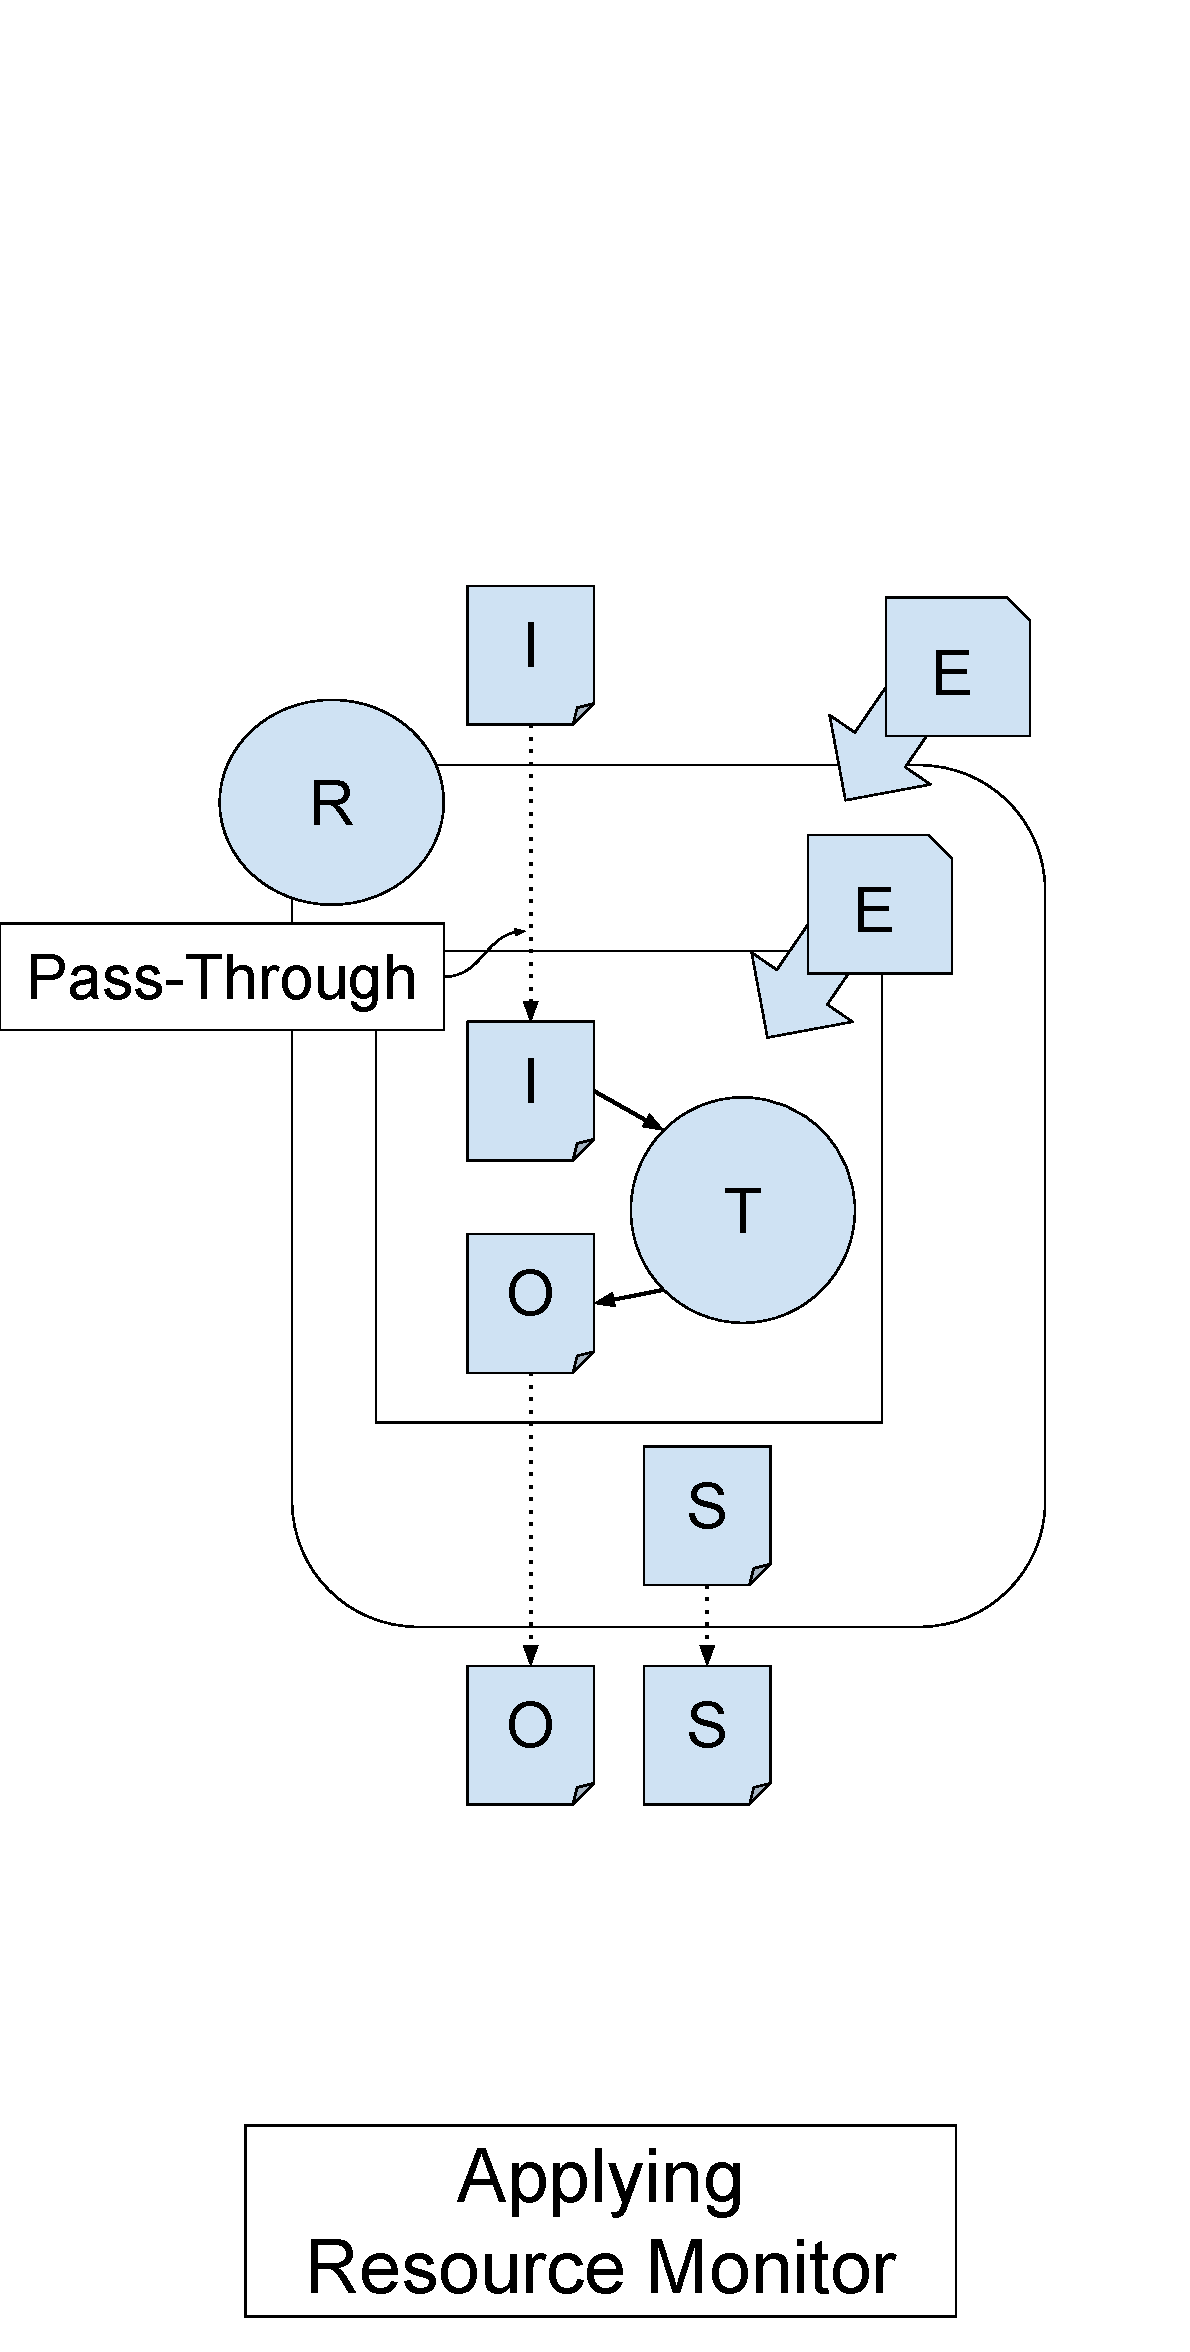
\includegraphics[width=\textwidth]{graphics/nested_sandbox_1_detail_wLlabel.pdf}
\end{minipage}
\begin{minipage}[t]{0.2\textwidth}
  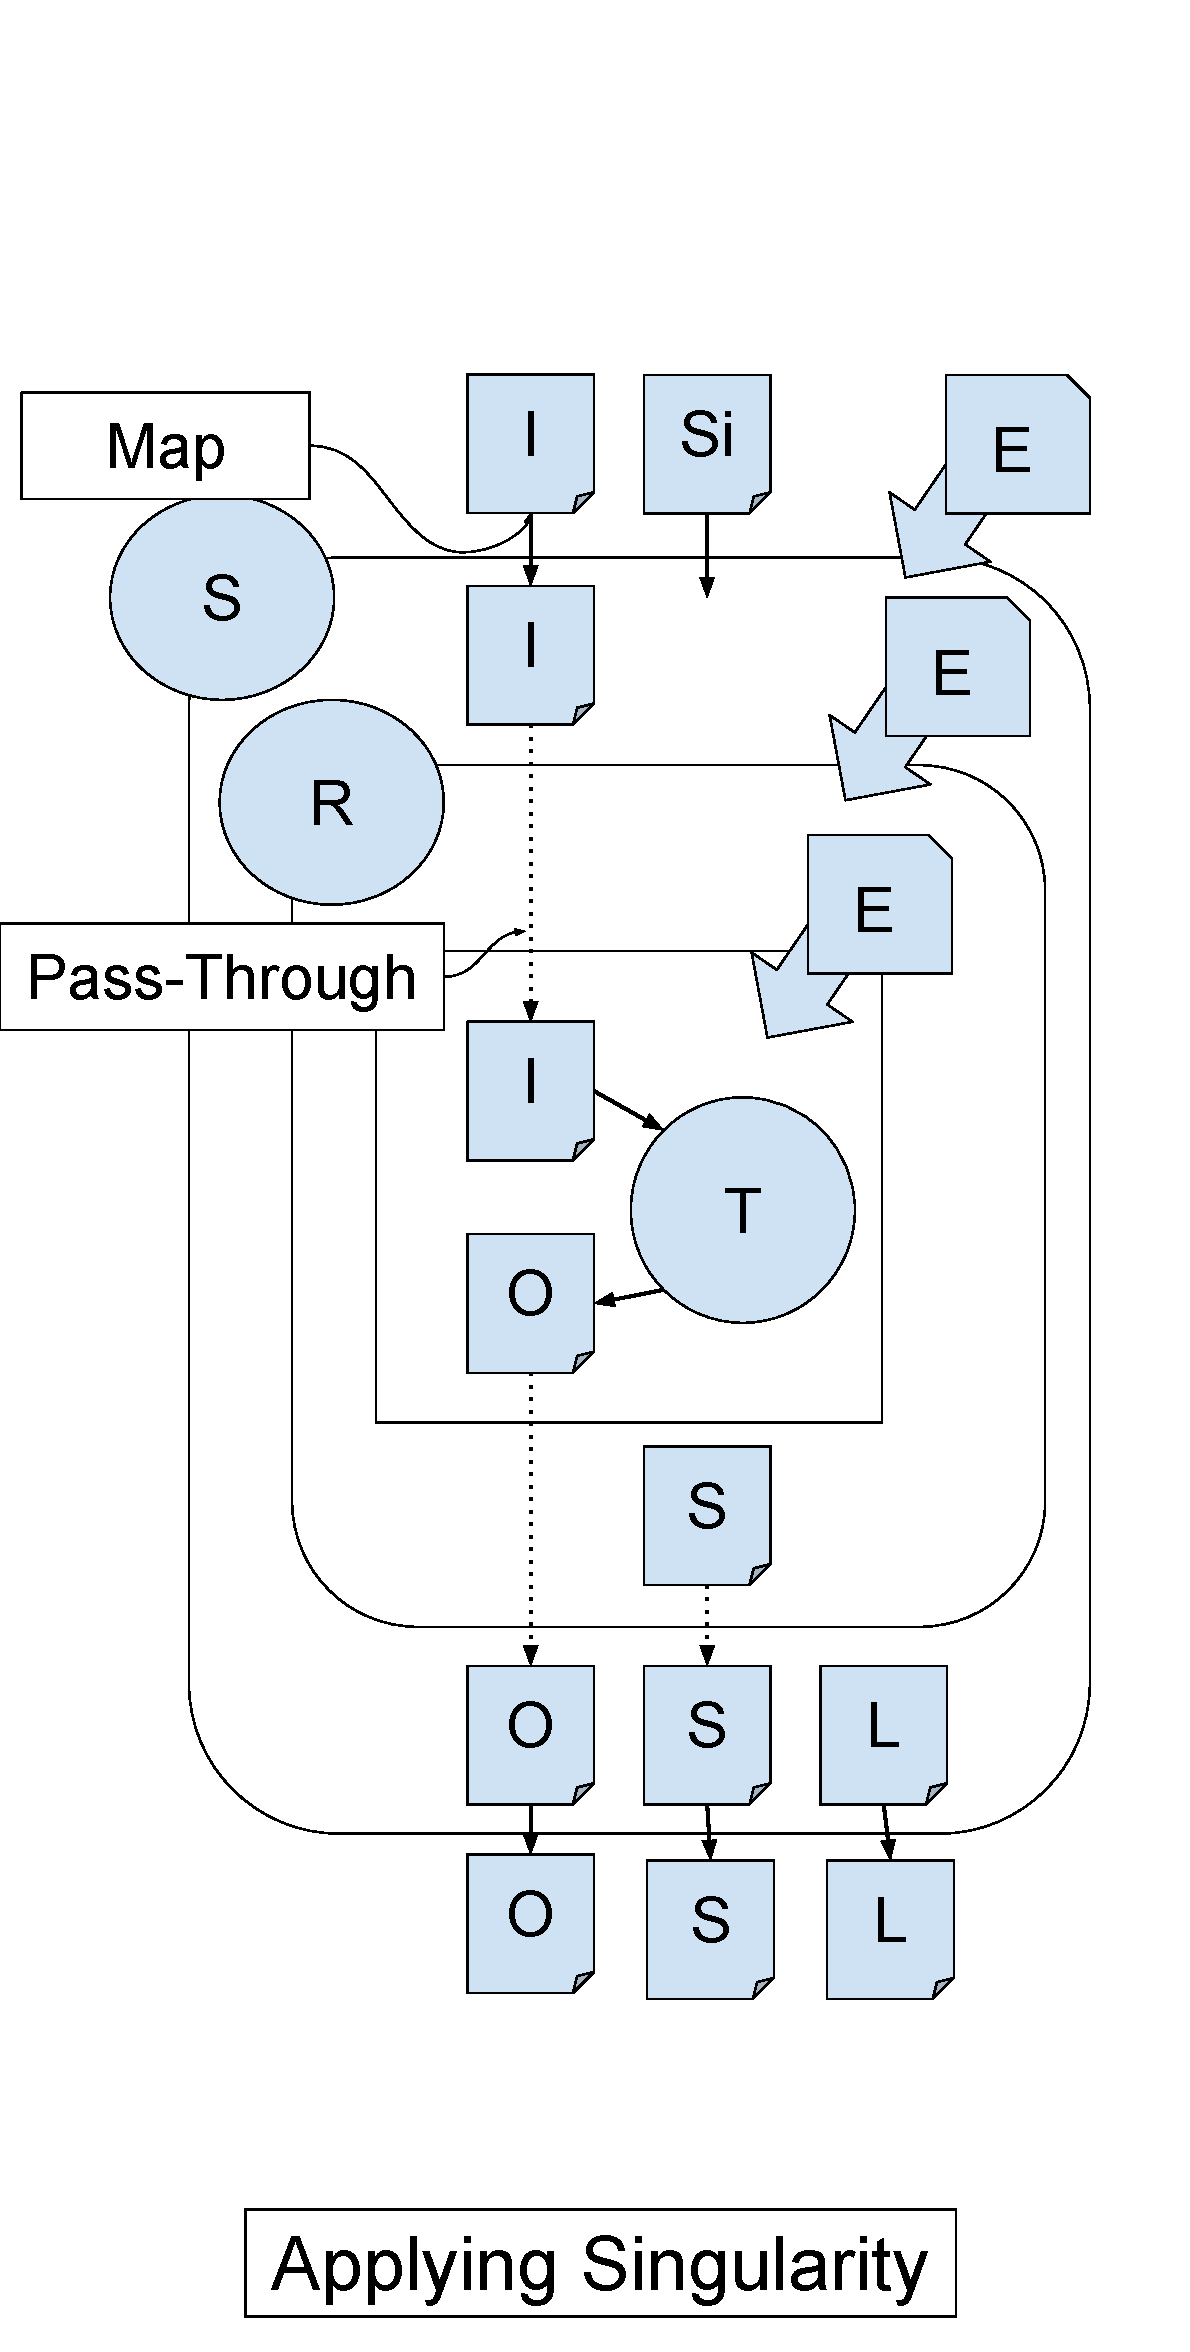
\includegraphics[width=\textwidth]{graphics/nested_sandbox_2_detail_wLlabel.pdf}
\end{minipage}
\begin{minipage}[t]{0.21\textwidth}
  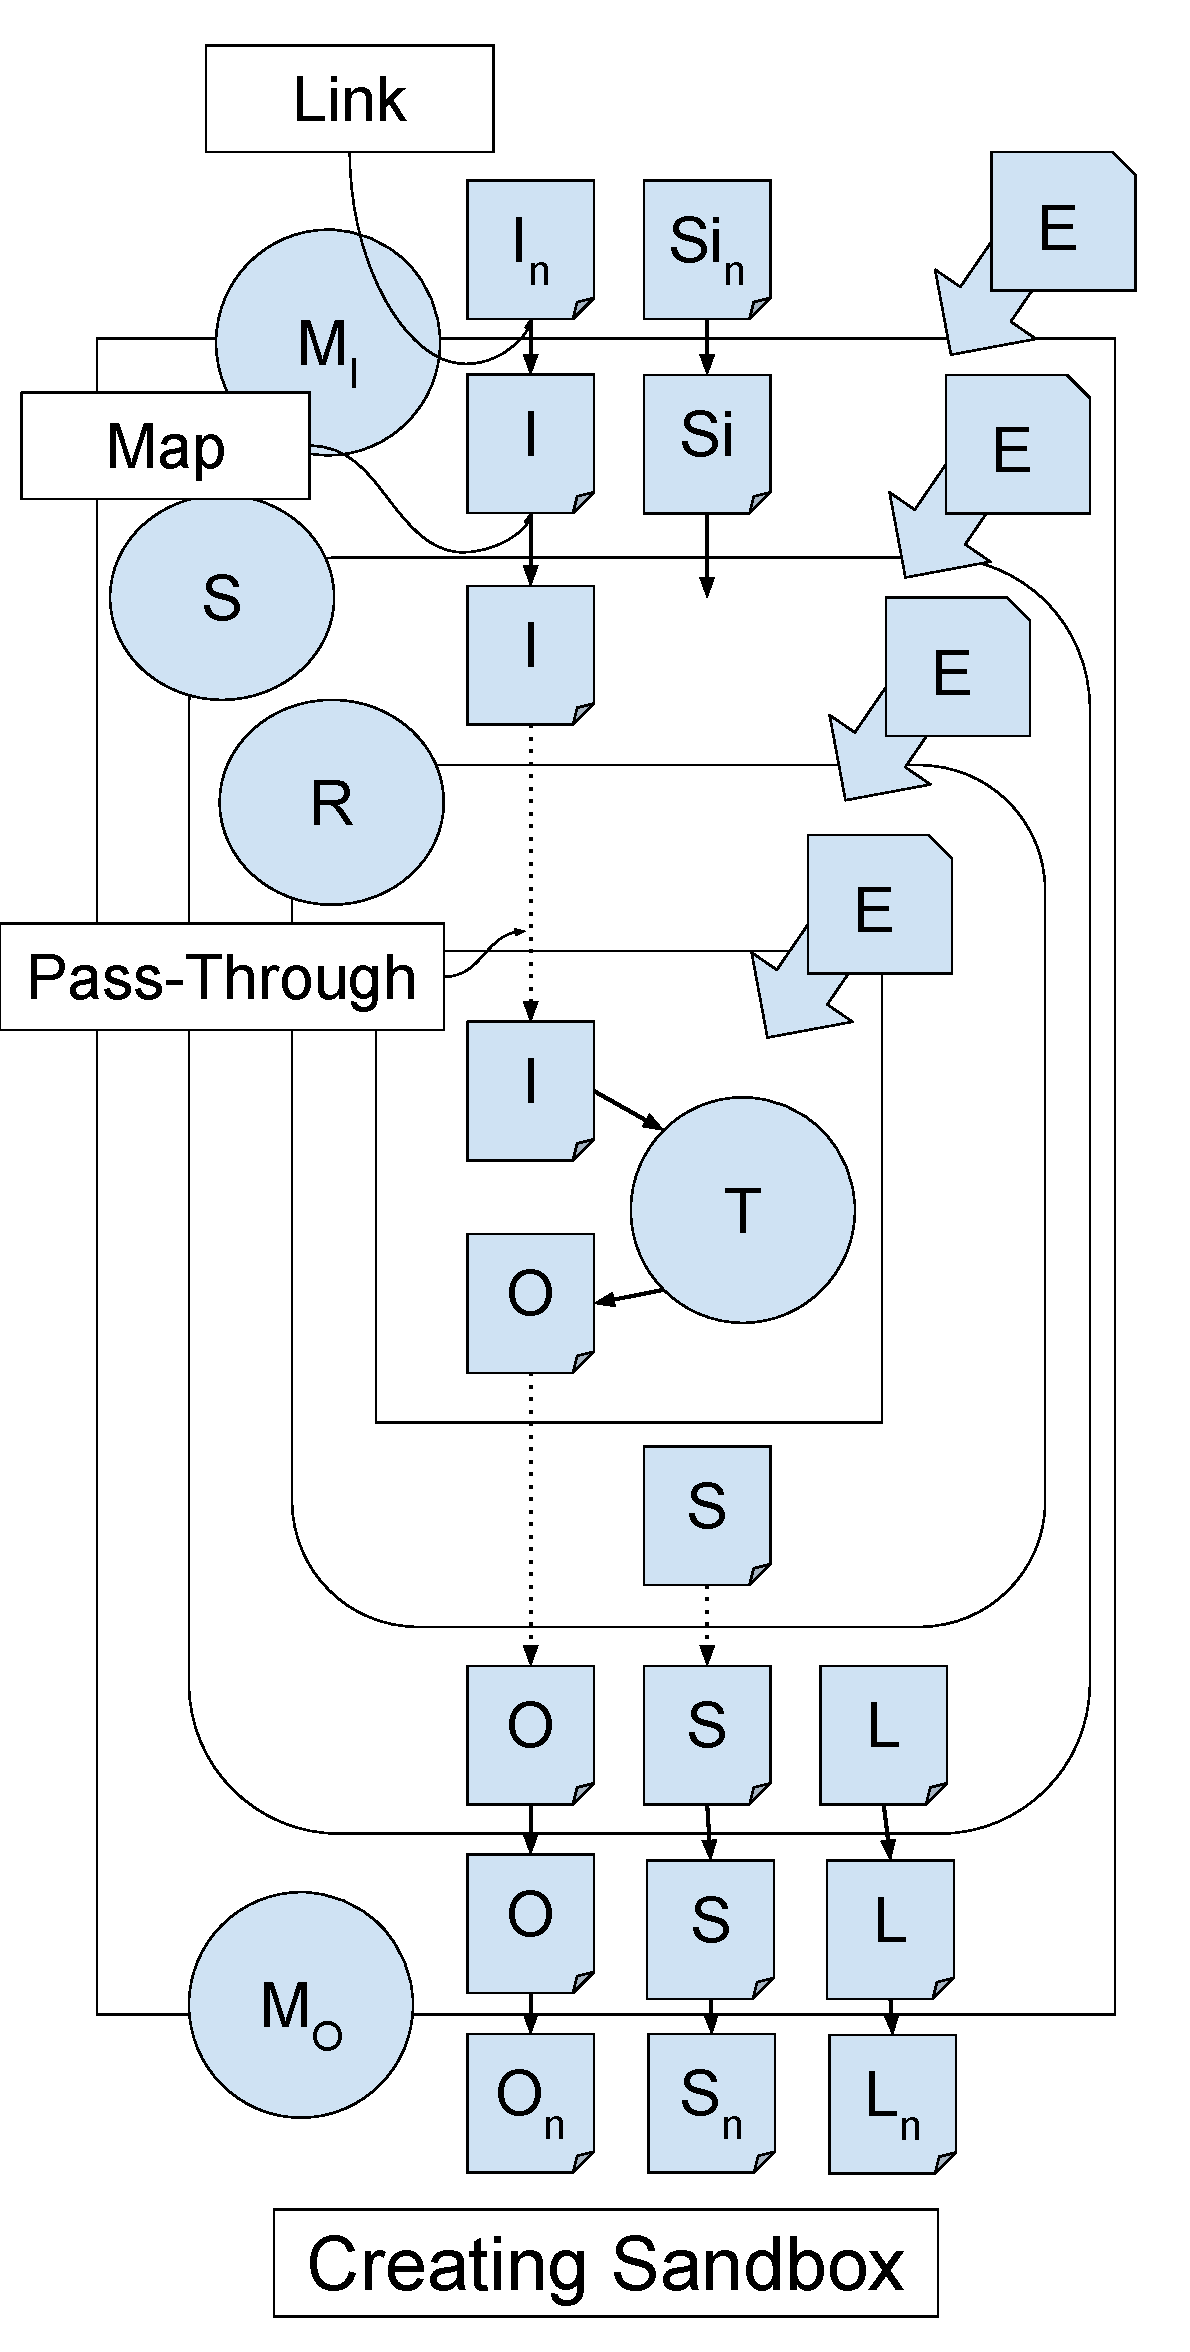
\includegraphics[width=\textwidth]{graphics/nested_sandbox_3_detail_wLlabel.pdf}
\end{minipage}
\begin{minipage}[t]{0.22\textwidth}
  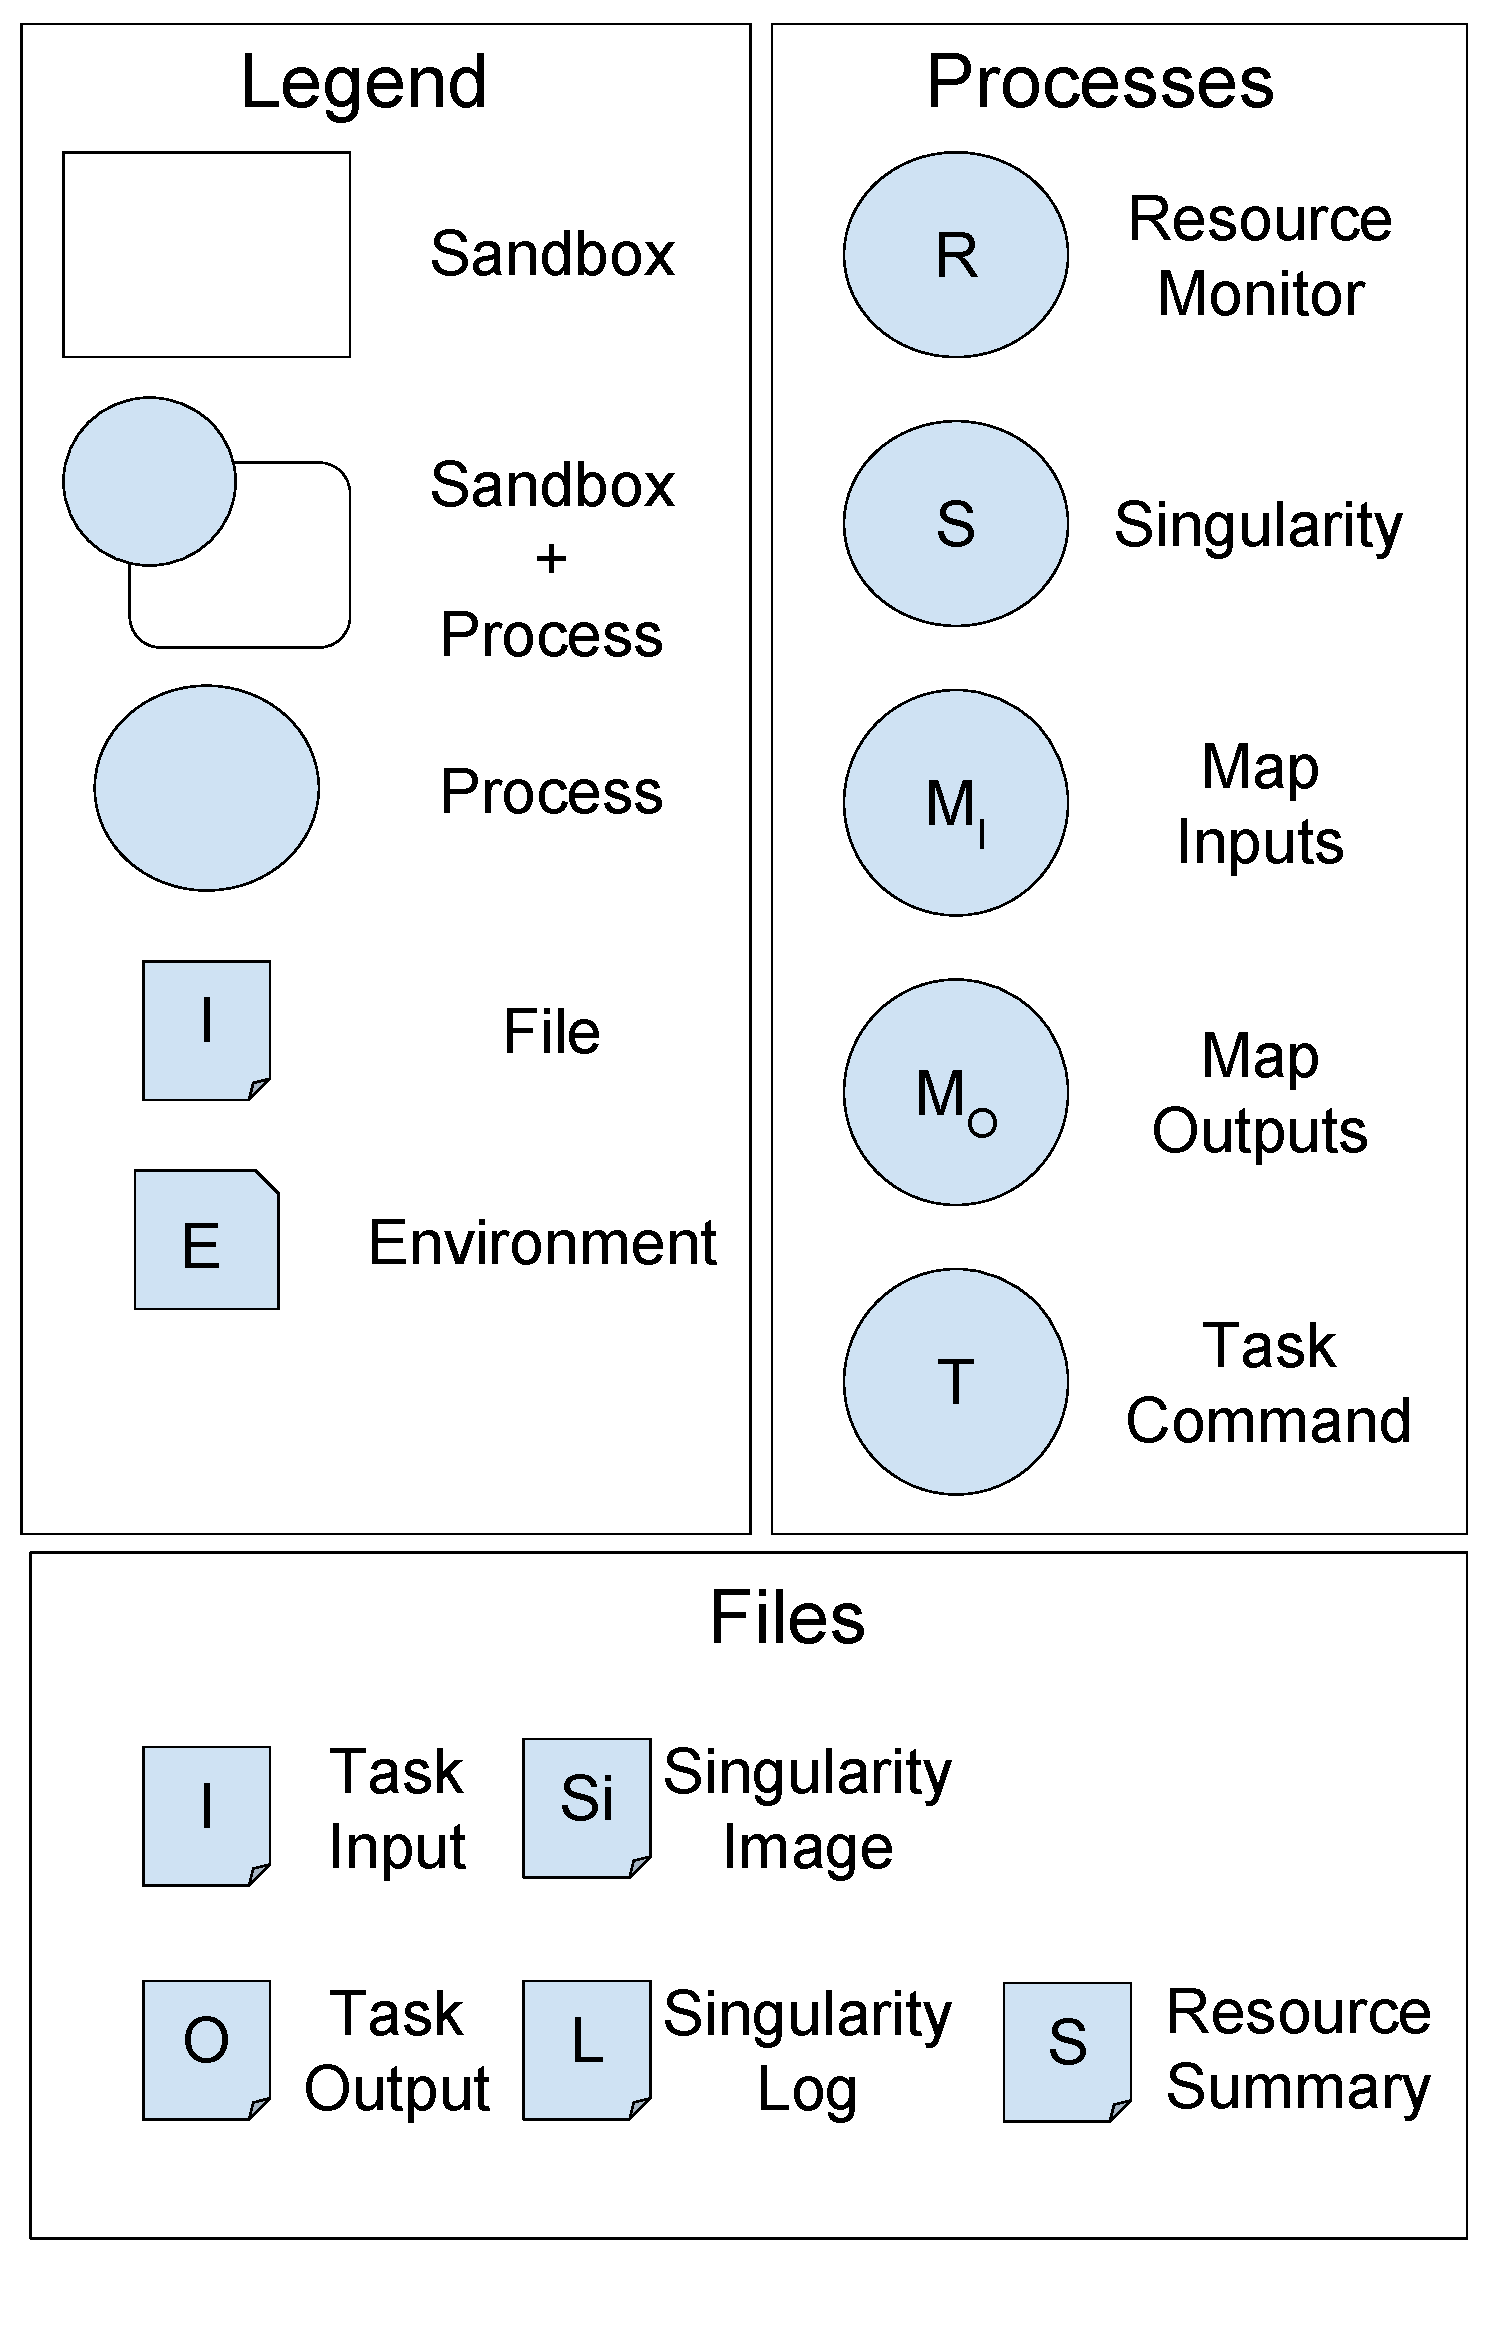
\includegraphics[width=\textwidth]{graphics/nested_legend.pdf}
\end{minipage}
\caption{Evolution of task as transformations are applied.} 
\small
\emph{ 
Starting from the left,
we have the initial task 
with a single input and output. 
Next, a resource monitor is applied which 
passes through the original files, 
but also creates a summary of the resources used.
After the resources monitor, a Singularity container
is used to provide a consistent operating system,
requiring a image to run from and creating a log.
Finally, a sandbox is created to isolate execution, 
limiting file access when singularity 
maps the current directory.
}
\label{figure:wrapping-of-task}
\end{figure*}

\subsection{Environment Transform}

Regardless if a submit script, 
container, or virtual machine 
is used to run a task, 
there is often a need for configuration 
just prior to task execution. 
This is necessary in cases such as
redirecting environment to reference data,
configuring variables to include new libraries
(such as {\tt LD\_PRELOAD}),
or specifying a precise version of Java
(by setting Java home and library paths).
These types of transformation rely on the 
${pre}$ command to initialize the environment. 
This can also be done using
the ${environment}$ dictionary, though these
value are directly exported and do not 
allow for nuanced initialization.

\subsection{Failure Handling Transform}

A transform that analyzes and handles errors at the task execution site
allows for evaluations of the environment where the error occurred.
Running evaluations only on failure limits the overhead 
on normal tasks and lessens the analysis burden of the user.
This is used in 
determining software configuration/version incompatibilities, 
verifying if failure was due to limited resources, 
analyzing output files to prevent corrupted output,
or process core-dumps into stack traces. 
Regardless of workflow size,
automating error handling helps to handled errors
allowing the user to analyze and address problems quickly. 
The error handling generally relies on the $post$ to 
perform analysis based on the reported
exit code or outputs.

\section{Case Studies}


\subsection{Resource usage in a Container}
Resource monitoring helps to build an understanding of how
a task behaves to accurately assign resources. 
If the task requires a container for execution, the 
resources utilized may be mischaracterized. 
As a result, it is useful to be able to separate the
resource utilization of the task and the container.
To do this, we first applied a 
resources monitor transformation to the task
which will measure the resources used only
by the task.
Second, we applied the container transformation
that allows for the application to run on 
different platforms.

The definitions of these transformations can
be seen earlier in \Cref{sing-wrap} and \Cref{json-file}
for Singularity and the resource monitor respectively.
To visualize the complexity that occurs when combining these
\Cref{figure:wrapping-of-task} illustrates each transformation.


\begin{framed}
\noindent
{\small makeflow bwa.mf --apply rmonitor.jx --apply singularity.jx}
\end{framed}

Using the above {\tt makeflow} call, we executed a workflow 
that runs BWA\cite{pmid20080505}.
This workflow partitions a large query and runs 
each chunk concurrently. 
This workflow was used as the basis to evaluate 
nesting the resource monitor and Singularity.
This workflow was run in four configuration,
both Singularity and the resource monitor,
just Singularity,
just the resource monitor,
and the workflow with task sandboxes.
We can examine the distribution of task
execution time under these different 
configuration in \Cref{figure:nest-task}
and see that there is minimal additional
overhead for each transformation.
For these runs, Singularity utilized
an image on a shared filesystem to
limit the sandbox creation time,
which can also be accomplished using
a link. In situations with no shared
filesystem the image is transferred
and affects performance.


\begin{figure}[h]
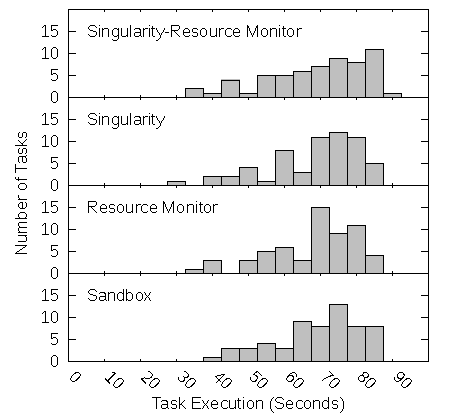
\includegraphics[width=\columnwidth]{graphics/divide_hist.pdf}
\caption{Histogram of task execution with nested transformations.}
\small
\emph{The distribution of task execution grouped by applied
transformations. 
The first configuration runs the resource monitor inside of
a Singularity, the second runs just Singularity,
the third runs just the resource-monitor, and the last
runs the task inside of an application sandbox.
We see that the distribution of execution
time is consistent between runs, and the amount of 
transformation overhead is minimal.
}
\label{figure:nest-task}
\end{figure}



\subsection{Failure Analysis}

When moving between sites or changing data
it is possible that an application can intermittently
fail causing a core-dump.
These core-dumps are unwieldy to move around and 
provide limited insight into the cause of the failure
and its environment. 

To address this we wrote a transformation that analyzes 
a core-dump at the execution site, and sends back the
resulting stack trace that is produced by GDB (GNU Project Debugger).
This transformation provides several keys benefits.
The first is that it allows for automated analysis of
core-dump failures for the user. Performing this in the 
execution sandbox provides early resolution about the
app that failed and which task created it.
Also, core-dumps are bloated and 
contain all of the memory and stack,
which are consolidated considerably in
a stack trace. 
This consolidation limits the amount of data 
transferred back to the user. 


Enabling the capture of core-dumps depends
on your systems default settings.
A common default uses the "core" prefix for
core dumps, but also limits their size. 
To accommodate this, we set the $ulimit$
to unlimited. After execution, if a 
core-dump was created we process it using GDB.
This creates a stack trace that condenses
the program failure.
We implemented this transformation as 
seen in \Cref{stacktrace}.

\begin{figure}[H]
\begin{framed}
\small
\begin{verbatim}
define StackTrace(T) {
 "command" : [
  "pre" : ["ulimit -c unlimited"],
  "cmd" : "./" + T.script,
  "post": ["gdb " + T.command{cmd} +
         "core* -ex bt > stack."+ T.ID ,
           "touch stack." +T.ID]
 ]
 "outputs" : T.outputs+ ["stack."+T.ID]
}
\end{verbatim}
\end{framed}
\caption{Stack Trace Transformation}
\small
\emph{The stack trace transformation allows a user
to capture a core-dump of a failed task and 
convert it into a stack trace. 
This is done by setting the ulimit 
to allow the full core-dump, running the script,
and then analyzing the core-dump with GDB.
The step of touching the stack trace
file prevents non-failed tasks from missing output.}
\label{stacktrace}
\end{figure}

To evaluate this we wrote an application
that
allocates 1MB of memory and then
fails roughly 20 percent
of the time, creating a core-dump. 
We scaled this experiment to see the 
difference of sending the 
stack trace instead of the core-dump.
As expected, we say differences of
several orders of magnitude of transfers,
reducing as much as 2.4 GB down to 0.5MB.
%\Cref{table:core-dump} shows a comparison
The table below shows a comparison
of workflows from 10 tasks up to 10000.
Using this technique on larger memory
intensive applications would yield 
more significant reductions.

%\begin{figure}
\begin{center}
\begin{tabular}{| r | r | r | r |}
\hline
\multicolumn{1}{|c|}{Workflow} & \multicolumn{1}{|c|}{Failed} & \multicolumn{1}{|c|}{Total Core} & \multicolumn{1}{|c|}{Total Stack} \\
\multicolumn{1}{|c|}{Tasks}    & \multicolumn{1}{|c|}{Tasks}  & \multicolumn{1}{|c|}{Dump Size}  & \multicolumn{1}{|c|}{Trace Size} \\ \hline
10 & 4 & 3.7MB & 0.8KB \\ \hline
100 & 24 & 28.6MB & 6.4KB\\ \hline
1000 & 174 & 214.9MB & 48.8KB \\ \hline
10000 & 1957 & 2.4GB & 553.1 KB \\ \hline
\end{tabular}
%\caption{Comparison of Raw Core-dump and Stack Trace data size.}
%\label{table:core-dump}
\end{center}
%\end{figure}


\subsection{Complex Software Configuration}

In scientific computing, researchers often construct
and rely on a complex stack of analysis tools
which are constructed over
months to years of work and configuration.
The resulting complexity often prevents researchers from
scaling up or sharing their configuration with
collaborators.
There are several tools and solutions that exist
to address this such as containers and build management
tools (like Nix\cite{Dolstra:2004:NSP:1052676.1052686} or 
Spack\cite{Gamblin:2015:SPM:2807591.2807623}).
This problem becomes more complex when the selected
solution is not supported on a different platform,
such as different container support or
required installation permissions (super-user).
For this reason we selected VC3-Builder\cite{tovar-ic2e-2018},
which is a user-level environment specification
and construction tool.

As an example of complex software we use MAKER\cite{pmid18025269},
a bioinformatic analysis pipeline which relies
on 39 separate packages and a installed size of 4.2G.
A MAKER installation requires careful
dependency management as several tools rely
on hard-coded, installation specific paths
and installing by hand can take several hour.
As a result, MAKER is often limited to a single
carefully configured site.
This is addressed with VC3-Builder and
we want to leverage this to use MAKER 
on several sites for one workflow.

The transformation for VC3-Builder often
simply invokes {\tt vc3-builder},
specifying the required dependencies,
and passing the command.
However, because of MAKER's complexity several
required packages have restrictive licenses
requiring the user 
pass and unpack the libraries.
In \Cref{vc3-builder}, we can see a file,
{\tt manual-distribution.tar.gz}, which
contains the restricted packages.
Using $pre$, we are able to set up the
correct directory structure,
unpack the manual packages,
and prepare for {\tt vc3-builder}.


\begin{figure}
\begin{framed}
%\small
\begin{verbatim}
define VC3-Builder(T) {
 "inputs" : T.inputs + ["vc3-builer",
            "manual-distibution.tar.gz"]
 "command" : [
  "pre" : [ "mkdir -p vc3-distfiles",
            "cd vc3-distfiles",
            "cp ../manual* ./",
            "tar xzvf manual*",
            "cd .."],
  "cmd": "./vc3-builder --require maker"
         + T.script, ]
 "resources":{
  "cores" : 4,
  "disk"  : T.resources{"disk"} + 4G,
} }
\end{verbatim}
\end{framed}
\caption{VC3-Builder Transformation}
\small
\emph{VC3-Builder is typically  
self-contained, and the specified
$cmd$ is sufficient for most software.
MAKER, however, relies on several libraries
with restricted licenses that must be
provided by the user. 
As a result, the transformation must
create the install structure and 
extract these libraries to the correct
location prior to VC3-Builder.
We specify cores for the make threads and 
increase the disk for the installation.
}
\label{vc3-builder}
\end{figure}

This workflow was executed using Makeflow
and distributed with Work Queue\cite{wq-python-pyhpc2011},
a master-worker execution platform. 
Workers were created on each target site,
and tasks were distributed as worker were 
scheduled.
To show the flexibility of transformations,
workers were created on Stampede2,
Jetstream, and HTCondor.
The table below shows the task execution
for each system, 
all of which were calculated using a single workflow.


%\begin{figure}[h]
\begin{center}
\begin{tabular}{| c | r | r | r |}
\hline
Build Time
  & \multicolumn{1}{|c|}{Stampede2} 
%  & \multicolumn{1}{|c|}{SGE} 
  & \multicolumn{1}{|c|}{Jetstream} 
  & \multicolumn{1}{|c|}{HTCondor} \\ \hline
 (HH:MM) & 01:29 & 00:22 & 00:30 \\ \hline
\end{tabular}
%\caption{MAKER build-times using VC3-Builder on several platforms.}
%\label{table:vc3-build-time}
\end{center}
%\end{figure}

\section{Related Work}

As we are looking at workflow 
transformations, it is important to look
at some of the major challenges of distributed
computing\cite{4404805},
which includes reproducibility, 
portability,
and flexibility, and 
how other workflow management systems
approach them.
Swift\cite{swift} programming language 
uses an $app$ to define a program's invocation.
Nesting apps could be similar, 
but the level of
specification used does
not address many of the
issue mentioned earlier, such
as name collisions, command
nesting, and execution evaluation.
Instead Swift focuses on compiler-like
optimizations for grouping work\cite{Armstrong:2014:CTM:2683593.2683627}.
Pegasus\cite{pegasus} focuses on planning the
execution prior to submission.
This allows for more strict
adherence to quota limits and attempts
to leverage the maximal parallelism,
even across multiple sites\cite{chen2011constraints}.
Pegasus allows for changes to a
workflow, but does so internally by clustering
tasks\cite{chen2013balanced, chen-tcc-2015, chen-fgcs-2014}, spawning clean-up
tasks to remove files\cite{cleanup_algo}, and 
restructuring the workflow\cite{cluster_dep}.

We also see similar work aimed at 
supporting containers natively.
For these systems to support containers,
there was a necessary level of work to abstract their applications,
design the interface, and then implement it
such that it works on a wide range of tasks
\cite{wq-docker-vtdc15, containers-sciencecloud-2018,7092947,7600178}.
Though this can deliver consistent execution,
the embedded nature of this implementation makes
it difficult for users to tailor the execution
to their needs/specifications and must be
managed.
This support must change to address
the available containers on a particular site,
such as 
Docker\cite{Merkel:2014:DLL:2600239.2600241},
Singularity\cite{Singularity}, 
CharlieCloud\cite{Priedhorsky:2017:CUC:3126908.3126925},
or extend to support functionality like Slacker\cite{194430}.


\section{Conclusion}

In the complex intersection of scientific
workflows and unique compute sites,
a solution was needed to allow for
quick flexible workflow transformations.
We introduced an algebra that formalizes 
task and workflow transformations. 
In conjunction with the formalization,
we also defined the sandbox model of execution
which allows these transformation to be applied,
but stay distinct in execution. 
We discussed several 
complications when designing for real workflows,
and explained how we addressed them, such as 
file remapping, differentiating command parts,
and clearly handling resources and environment.
These methods were evaluated with three case studies.
First, we nested a resource monitor in a container
with consistent performance.
Next, we captured and processed a task core-dump
limiting the analysis and file transfer needed.
Lastly, we executed a workflow across several sites running a 
complex application seamlessly.
Using workflow transformations
we were able to quickly transform workflows to fit 
unique configurations, without modifying the core work.



\section{Reproducibility Data}

In an effort to provide consistent, reproducible results outlined are the
resources utilized in this paper and where they can be found.
Specific commits are mentioned to provide the exact version that was used.

The first is CCTools, which is an open-source distributed computing 
tool kit, containing Makeflow and Work Queue:
\begin{framed}
\noindent
{\small https://github.com/nhazekam/cctools/commit/7ab0645}
\end{framed}

Second is the source for some of our example workflows,
particularly BWA using in the first case study:
\begin{framed}
\noindent
{\small https://github.com/cooperative-computing-lab/makeflow-examples/commit/600e13b}
\end{framed}

The last case study uses VC3-Builder, found here:
\begin{framed}
\noindent
{\small https://github.com/vc3-project/vc3-builder/commit/dc285f9}
\end{framed}

All of the workflows, transformations, and auxiliary
programs used to produce this paper, include the tex, found here:
\begin{framed}
\noindent
{\small https://github.com/cooperative-computing-lab/workflow-algebra-paper/commit/be9d1e4}
\end{framed}
\noindent
As this is self-referential the final commit may be different.


All of these repositories are open source and contain Makefiles
and instructions on how to build and run them.



\section*{Acknowledgment}

This work was supported by part by National Science Foundation grant ACI-1642409.


\bibliographystyle{IEEEtran}
\bibliography{otherpapers,cclpapers}

\end{document}